\chapter{Introducción}
\label{ch:intro}

En este capítulo, se introduce al lector en el dominio de las apuestas deportivas en Internet y se presenta el terminal elegido como plataforma para la aplicación de apuestas, resultado del presente trabajo de fin de carrera.

\section{Apuestas por Internet}

Actualmente las apuestas tienen gran aceptación comercial en todo el mundo. En España ya existe una tradición de bastantes años por la quiniela y la lotería. En la quiniela, por ejemplo, nunca sabemos por anticipado cuánto cobraremos en caso de acierto ya que depende del número de participantes que hayan acertado el resultado de la jornada de la Liga Profesional de Fútbol. Un acierto de 13 resultados puede convertirse en una gran decepción por el premio conseguido si junto con nosotros han acertado el resultado otras 10000 personas. Sin embargo, si eres el único acertante ya no tienes que repartir el premio. 
 Hace unos pocos años proliferaban las casas de apuestas tradicionales. En estas el apostante cruza su apuesta directamente contra la propia casa. En un típico ejemplo tenemos las clásicas carreras de caballos sobre las que se apuesta sobre un caballo ganador. La casa de apuesta tradicional se limita siempre a cubrir nuestras apuestas asesorados por expertos y siempre con el objetivo de asegurar ganancia sobre el total de las apuestas abierta, por ejemplo, mediante comisiones. 
En los últimos años hemos sido testigos de la llegada de las llamadas casas de intercambio. 
Las casas de intercambio añaden un nuevo concepto en el mundo de las apuestas. Los usuarios realizan las apuestas sobre los eventos y entre ellos mismos se cubren las apuestas, es decir, los apostantes pueden realizar apuestas a favor o en contra de los eventos. 
 En este caso, la casa de apuestas hace de intermediario obteniendo un porcentaje en la ganancia del apostante, una comisión que se calcula sobre la ganancia neta obtenida por el usuario.
 Las ventajas para los clientes de las casas de apuestas de intercambio con respecto a las tradicionales son:
\begin{itemize}
	\item Las comisiones son menores que las correspondientes a una casa de apuestas tradicionales.
	\item Cuanto mayores sean las cantidades apostadas, mayor será la comisión que se lleve la casa de intercambio, es por eso que no suelen existir límites en las cantidades a apostar en contra de las casas de apuestas tradicionales siempre y cuando se cubra una apuesta a favor con otro en contra.
\end{itemize}
Pero como en toda comparación siempre hay desventajas para el cliente: 
\begin{itemize}
	\item Normalmente, debido a las nuevas posibilidades de apuesta de las casas de intercambio se requieren conocimientos avanzados y una mayor experiencia para obtener beneficios en contraposición a la simplicidad que ofrecen las casas de apuestas tradicionales.
	\item En las casas de intercambio son los propios usuarios los que proponen sus apuestas y los mercados tardan más tiempo en abrirse. Se necesita que aparezca un apostante para abrir el mercado. Entendemos por mercado el evento deportivo por el cual podemos apostar a favor o en contra. Por ejemplo, en un partido de tenis apostar por cuál de los dos jugadores va a ganar. En las casas de apuestas tradicionales es la propia casa la que establece las cuotas abriendo los mercados más rápidamente.
\end{itemize}

Debido a la aparición de estas casas de intercambio, aparecen una nueva modalidad para realizar apuestas: el poder realizar apuestas en contra de un evento (\emph{lay}) . Esta es la principal diferencia clara con las casas de apuestas tradicionales donde sólo se pueden realizar apuestas a favor (\emph{back}) de un evento.
 Con esta nueva modalidad para realizar apuestas se facilita a los apostantes la tarea para realizar \emph{trading}, concepto que desarrollaremos en el siguiente apartado.

 \subsection{Apuestas a favor (\emph{back}) y en contra (\emph{lay})}
 
   Para un mejor entendimiento y comprensión de la temática de este trabajo de fin de carrera, definiremos los principales conceptos en una apuesta:
 \begin{itemize}
 \item \emph{Bankroll}: es la cantidad de dinero o capital  que estamos dispuestos a jugar. Lógicamente tendremos que administrarlo de la mejor manera posible, minimizando las pérdidas en caso de perder una apuesta y maximizar las ganancias de una apuesta ganadora. La disciplina y el conocimiento del mercado son las mejores aliadas de nuestro \emph{bankroll}. La mayoría de las casas de apuestas por Internet nos regalan un mínimo \emph{bankroll} para animarnos a participar en ellas.
 \item \emph{Stake}: es la cantidad de dinero que apostamos por un resultado. Es decir, apostar 10\euro{} a que gana el Sevilla F.C el campeonato de la Liga Profesional de Fútbol tendría un \emph{stake} de 10\euro.
 \item \emph{Odds}: es la cuota de una apuesta y refleja la probabilidad de éxito ese evento. Normalmente se representa de forma decimal aunque se puede encontrar de forma fraccional. Por ejemplo se paga una cuota de 1 a 3 que Fernando Alonso gane el mundial de Fórmula 1. Nos refleja que Fernando Alonso tiene más probabilidades de ganar el campeonato que no ganarlo.
 \item Beneficio: es la ganancia que obtenemos de una apuesta ganadora. Dependiendo si nuestra apuesta es a favor o en contra el cálculo es el siguiente:
 
 	Apuesta a favor:
	
 \begin{displaymath}
 Beneficio_\emph{back} = (stake \times odd) - stake  
\end{displaymath}

	Apuestas en contra:
	
 \begin{displaymath}
 Beneficio_\emph{lay}  =  stake  
\end{displaymath}

\item Pérdida o riesgo: lógicamente lo opuesto al beneficio. Lo que todo apostante quiere evitar o minimizar. La pérdida también se puede expresar mediante el término riesgo. Igual que el beneficio su cálculo depende si estamos apostando a favor o en contra de un evento.

	Apuesta a favor:
	
 \begin{displaymath}
 Riesgo_\emph{back} = stake  
\end{displaymath}
	
	Apuesta en contra:
	
 \begin{displaymath}
 Riesgo_\emph{lay} = stake - (odd \times stake)
\end{displaymath}

\item \emph{Yield}: expresado en porcentaje. Nos indica el beneficio obtenido del total apostado. Es lo que diferencia a un buen apostador del resto. El cálculo es el siguiente:
\begin{displaymath}
 Yield = (beneficio / total apostado) \times 100 
\end{displaymath}
\end{itemize} 


 
 \subsection{Trading}
 
 Se trata de apostar a favor y en contra sobre un mismo evento en distinto momentos para obtener así una ganancia segura en unos casos o minimizar la pérdida en otros.  Esta modalidad se puede realizar en la casa de apuestas tradicionales pero para ello necesitas usar varias casas.  Es decir, en una casa cubre la apuesta a favor de un evento mientras que otra casa ve más interesante cubrir la opuesta. Este término también se suele usar en operaciones financieras, como por ejemplo la Bolsa. También es posible realizarlo sobre varios eventos relacionados pero esta última opción resulta muy compleja a efecto de cálculos.
 
A continuación exponemos un ejemplo de caso típico de \emph{trading}. Nos basaremos en las apuestas deportivas sobre un partido de tenis.
 
 \begin{center}
    \begin{tabular}{| c | c | c |}
      \hline
      \hline
      \textbf{Players} & \textbf{A favor} & \textbf{En contra}\\
      \hline
      \hline
      Rafa Nadal & 2.5 & 2.75\\
      \hline
      \hline
      Roger Federer & 1.57 & 1.67\\
      \hline
      \hline
    \end{tabular}
  \end{center}


En la tabla podemos ver las cuotas a favor y en contra al inicio (\emph{odds}) de un partido de tenis entre Rafa Nadal y Roger Federer. La cuota a favor de Rafa Nadal está más alta que la de Roger Federer, con lo que no parte como claro favorito en el partido. En este ejemplo realizaremos una apuesta a favor de Rafa Nadal con un \emph{stake} de 50 \euro . Calculamos el beneficio que obtendríamos en caso de ganar Nadal.

  
\begin{displaymath}
  Beneficio_\emph{back} = (2.5 \times 50) - 50 =  75\euro  
\end{displaymath}

Por lo que tenemos 75\euro si ganal Nadal, en caso contrario:
 
 \begin{displaymath}
  Riesgo_\emph{back} = - 50 
\end{displaymath}

Tendremos una pérdida de 50\euro si pierde Nadal.

En el mundo de las apuestas, influyen todos los pequeños factores que al aficionado se les escapa. Supongamos que Nadal gana los dos primeros sets, esto desemboca en cambios en la tabla de apuestas. 

Vemos ahora que el mercado ha cambiado. Ahora la cuota de Nadal ha bajado claramente.
   
 \begin{center}
    \begin{tabular}{| c | c | c |}
      \hline
      \hline
      \textbf{Players} & \textbf{A favor} & \textbf{En contra}\\
      \hline
      \hline
      Rafa Nadal & 1.2 & 1.25\\
      \hline
      \hline
      Roger Federer & 5 & 6\\
      \hline
      \hline
    \end{tabular}
  \end{center}
  
  
  El mercado ha cambiado debido al resultado de los dos primeros set, Nadal ya es favorito pero queremos asegurarnos un beneficio seguro.
  
Para asegurar el dinero apostado anteriormente realizamos una apuesta en contra de Nadal. De tal forma que nos queda:

  \begin{displaymath}
  Beneficio_\emph{lay} = 60 
  \end{displaymath} 
  
   Obtenemos 60\euro si pierde Nadal.
   
   \begin{displaymath}
  Riesgo_\emph{lay} = 60 - (1.25 \times 60) = -15
  \end{displaymath} 
  
  Y un riesgo de 15\euro si gana Nadal.
  
En las apuestas siempre tenemos que tener en cuenta en factor de imprevisibilidad. No siempre ocurre todo como esperamos. En este caso, debido a que es un partido con dos jugadores de primer nivel, tenemos la ocasión de asegurar beneficios si apostamos en contra de Nadal. Aunque pueda parecer raro, siempre puede haber condiciones que afecten claramente a los resultados como por ejemplo una lesión de Nadal.
	 
Al final si gana Rafa Nadal obtenemos: 
   \begin{displaymath}
   75 - 15 = 50 
   \end{displaymath}
   
Si pierde Nadal y por tanto gana Roger Federar tenemos:
   
  \begin{displaymath}
  60 - 50 = 10 
  \end{displaymath}
       
   Con lo que estamos cubiertos ante cualquier resultado del partido. En ambos casos tenemos ganancias. 
   
   Recordemos que al principio del partido Rafa Nadal no era favorito pero hemos supuesto una apuesta a favor. El apostante puede realizar esta apuesta de forma aleatoria, al estilo de la lotería. Pero en estos casos hay que reducir el factor suerte tanto como podamos. Una manera de hacerlo es usar todos los datos que tengamos a mano, como estadística de enfrentamientos anteriores, momento de forma de cada uno \dots   
   
   En este ejemplo, el escenario expuesto es uno de los mejores casos que nos pueden dar ya que obtenemos beneficio en ambos casos. Pero puede suceder que hayamos apostado por un evento con demasiada confianza y luego en un futuro vemos que puede ser una ruina. En ese escenario, el objetivo prioritario sería minimizar la pérdida apostando en contra del evento en cuestión.

En el \emph{trading} se suele dar en dos escenarios típicos:
  
\begin{itemize}
	\item Ganancia segura.
	  Se suele llamar apuesta segura, es decir cualquiera que sea el desenlace del evento, obtenemos ganancia. La condición necesaria para ello es que la cuota de la apuesta a favor sea superior a la cuota de la apuesta en contra. 
	\item Minimizar la pérdida.
	   El mercado evoluciona de tal manera que la cuota de la apuesta en contra es mayor que la ya realizada a favor. En este caso lo que se persigue es minimizar la pérdida segura.
\end{itemize}
   
\section{Betfair}

 Debido al gran desarrollo de Internet en los principios de siglo empiezan a aparecer las primeras casas de apuestas online. Betfair\footnote{\url{www.betfair.com}}, Bwin\footnote{\url{www.bwin.com}}, Miapuesta.com\footnote{\url{http://www.miapuesta.com}} son ejemplos de casas afianzadas en Internet. Dentro de este grupo selecto aparece Betfair.

 Betfair fue fundado en Junio del año 2000. Es una de las primeras casas de apuestas online en ofrecer la modalidad de apuestas a favor y en contra de un evento. En el año 2007 la casa ya cuenta con más de 1.000.000 de usuarios generando un volumen de negocio de más de 50 millones de libras a la semana. Rápidamente se expande en más de 120 países de todo el mundo ofreciendo un portal web en 18 idiomas que gestiona más de 5 millones de transacciones al día. 

En el año 2007, Betfair es el primer portal de apuestas que ofrece un API\footnote{Application Programming Interface} de acceso a sus servicios. En líneas generales el API nos permite acceder a los servicios ofrecidos en su página web pero en aplicaciones desarrolladas por terceros. El API de Betfair lo explicaremos con más detalle en el capítulo \ref{ch:diseno}. Con esta estrategia se intenta enganchar a los desarrolladores para crear todo tipo de aplicaciones usando sus servicios web como base y que se adapten a cualquier dispositivo sea tanto un ordenador personal, agenda electrónica o dispositivo móvil. Como era de esperar, empezaron a surgir multitud de desarrollos, sobre todo dirigidas al sector de usuarios expertos en apuestas, donde se le ofrece al usuario más información, sobre todo matemática, a la hora de apostar por un evento.

\subsection{Organización de la información en Betfair}

 Betfair utiliza una estructura de eventos y mercados para representar las apuestas disponibles desde su portal. Un evento para Betfair es una actividad deportiva, por ejemplo un partido de fútbol. Un mercado es, sin embargo, un resultado por el que podemos apostar con cuotas asociadas. Un evento puede albergar varios eventos y mercados.Por ejemplo, dentro de la Liga Profesional de Fútbol tenemos el partido Real Madrid contra el Barcelona y la posibilidad de apostar por el equipo ganador de la competición. En este caso el eventos es el partido y el mercado el campeón de la competición. En la figura \ref{fig:eventoymercado} podemos ver un ejemplo claro de como se organiza la información en Betfair.
 
 \begin{figure} [h]
  \centering
    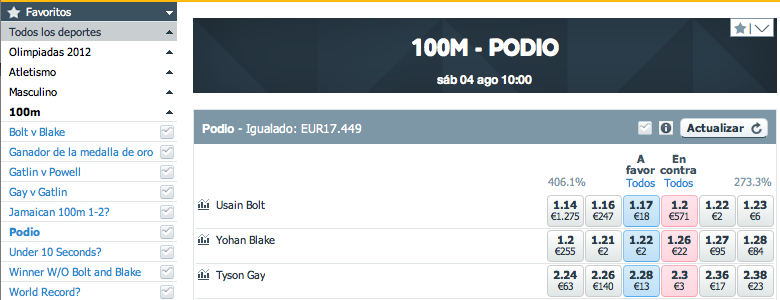
\includegraphics[width=0.95\linewidth]{./images/introbetfair.png} 
  \caption{Ejemplo de eventos y mercados en Betfair}
  \label{fig:eventoymercado}
\end{figure}

 Dentro del evento Olimpiadas, tenemos disponible el evento de los 100 metros lisos y la información del mercado acerca del ganador de la final.
 
\section{Apple y su terminal móvil iPhone}
 
Apple Computer, Inc. es una empresa estadounidense de tecnología informática fundada en 1976. Inició sus trabajos sobre los ordenadores personales en la década de los setenta con el ordenador Apple II y reinventó el ordenador personal en los ochenta con el Macintosh. Hoy en día, Apple es considerada como una de las principales empresas líderes en tecnología.

El 9 enero del año 2007 presenta su primer terminal móvil llamado \emph{iPhone}. Tal y como lo hizo años atrás en la industria musical, su terminal se hizo famoso en la industría de la telefonía móvil por su diseño, su sistema operativo \emph{iPhone OS} y la introducción de nuevas tecnologías como la pantalla táctil.

\begin{figure} [h]
  \centering
    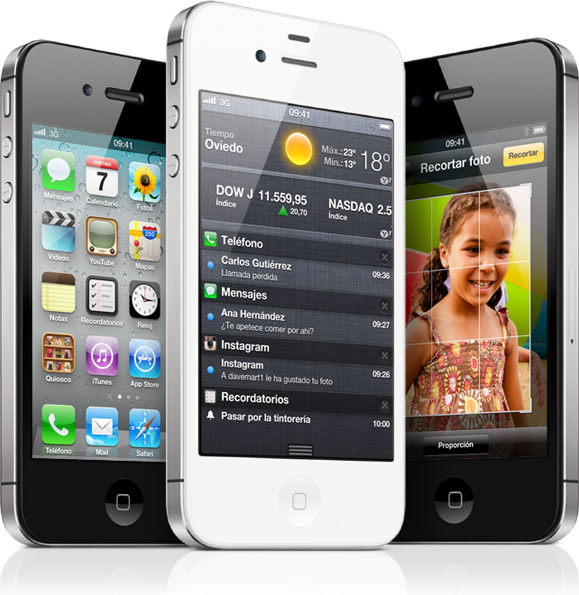
\includegraphics[width=0.6\textwidth]{./images/iphone4.jpg} 
  \caption{iPhone 4S}
  \label{fig:iPhone-4GS}
\end{figure}
  
  En marzo de 2008 Apple muestra una nueva versión del terminal con tecnología 3G y comunica el lanzamiento de su propia tienda de aplicaciones para el iPhone, la \emph{iTunes application store}. Para nutrir esa tienda de aplicaciones  lanza un conjunto de herramientas de desarrollo iPhone SDK\footnote{Software Development Kit} para todos aquellos desarrolladores que quieran participar en la misma. En el capítulo \ref{ch:diseno}  explicamos con más detalle dicho SDK ya que es una pieza clave en el presente trabajo de fin de carrera.
  
   Otro hito importante a destacar ocurre el 27 de enero de 2010. Apple amplía la familia de dispositivos con una tableta táctil de 10 pulgadas denominada \emph{iPad}. Misma filosofía pero ahora en formato de pantalla más grande. De la misma forma que evoluciona sus dispositivos, evoluciona el \emph{SDK} para ofrecer a los desarrolladores las herramientas necesarias para crear aplicaciones compatibles entre la familia de dispositivos. A partir de 2010 el sistema operativo de los dispositivos para a denominarse \emph{iOS}. 
    
  Hoy en día, Apple dispone de un catálogo de más de 500.000 aplicaciones disponibles en su tienda\footnote{Fuente: www.apple.com y http://148apps.biz/app-store-metrics/} y más de 316 millones de terminales vendidos por todo el mundo.\footnote{Fuente: www.apple.com} He aquí la importancia de la temática de este trabajo de fin de carrera, adaptar el acceso de los servicios de Betfair a una de las plataformas móviles más extendidas del mundo.     
   
\section{Objetivos}

 El objetivo que se pretenden cubrir con el actual trabajo de fin de carrera es el acceso a los servicios web de Betfair a través de la plataforma \emph{iOS} de Apple. Para ello hemos marcado una serie de hitos a alcanzar:
 \begin{itemize}
 	\item Explorar y adaptar el API de Betfair para la plataforma iPhone.
 	\item Posibilidad de navegar y apostar por eventos del portal betfair.com a través del terminal móvil.
	\item Asesorar al usuario sobre cuando realizar el \emph{trading} a las apuestas ya realizadas.
\end{itemize}

%%% Local Variables: 
%%% mode: latex
%%% TeX-master: "tfc-betfair-ios"
%%% TeX-PDF-mode: t
%%% ispell-local-dictionary: "castellano"
%%% End: 
